\documentclass[11pt]{article}
%\usepackage[firstpage]{draftwatermark}
\usepackage{times}
\usepackage{pdfpages}
\usepackage{fullpage}
\usepackage{url}
\usepackage{hyperref}
\usepackage{fancyhdr}
\usepackage{graphicx}
\usepackage{tabularx}
\usepackage{enumitem}
\setlist{nosep} % or \setlist{noitemsep} to leave space around whole list
\usepackage{indentfirst}
\usepackage{subcaption}
\usepackage{units}
\usepackage{bm}
\usepackage{algorithm}
\usepackage{algorithmic}

\usepackage{./math_bbing}


% Highlighting
\usepackage{color,soul}
\DeclareRobustCommand{\hlr}[1]{{\sethlcolor{red}\hl{#1}}}
\DeclareRobustCommand{\hlg}[1]{{\sethlcolor{green}\hl{#1}}}
\DeclareRobustCommand{\hlb}[1]{{\sethlcolor{blue}\hl{#1}}}
\DeclareRobustCommand{\hly}[1]{{\sethlcolor{yellow}\hl{#1}}}

\setcounter{secnumdepth}{4}
\graphicspath{{images/}}
\pagestyle{fancy}

% Conditional for notes
\newif\ifnotes
\notesfalse


\newcommand{\doctitle}{Wave Generation}

\newcommand{\docnumber}{\doctitle}

\addtolength{\headheight}{2em}
\addtolength{\headsep}{1.5em}
\lhead{\docnumber}
\rhead{}

\newcommand{\capt}[1]{\caption{\small \em #1}}

\cfoot{\small Brian Bingham \today \\ \thepage}
\renewcommand{\footrulewidth}{0.4pt}

\newenvironment{xitemize}{\begin{itemize}\addtolength{\itemsep}{-0.75em}}{\end{itemize}}
\newenvironment{tasklist}{\begin{enumerate}[label=\textbf{\thesubsubsection-\arabic*},ref=\thesubsubsection-\arabic*,leftmargin=*]}{\end{enumerate}}
\newcommand\todo[1]{{\bf TODO: #1}}
\setcounter{tocdepth}{2}
\setcounter{secnumdepth}{4}

\makeatletter
\newcommand*{\compress}{\@minipagetrue}
\makeatother

%\renewcommand{\chaptername}{Volume}
%\renewcommand{\thesection}{\Roman{section}}
%\renewcommand{\thesubsection}{\Roman{section}-\Alph{subsection}}

\begin{document}
% List of new commands
% bbing 06-11-98

%\newcommand{\spacing}[1]{\renewcommand{\baselinestretch}{#1} \normalsize}

% Degree symbol within text
\newcommand{\degrees}{$^{\circ}$}
\newcommand{\CRlb}{Cram\'{e}r Rao }

\newcommand{\btab}{\begin{tabular}}
\newcommand{\etab}{\end{tabular}}

\newcommand{\bfig}{\begin{figure}}
\newcommand{\efig}{\end{figure}}

\newcommand{\beqn}{\begin{equation}}
\newcommand{\eeqn}{\end{equation}}
\newcommand{\bdm}{\begin{displaymath}}
\newcommand{\edm}{\end{displaymath}}

\newcommand{\bearray}{\begin{eqnarray}}
\newcommand{\eearray}{\end{eqnarray}}
\newcommand{\Bearray}{\begin{eqnarray}}
\newcommand{\Eearray}{\end{eqnarray}}

\newcommand{\bgat}{\begin{gather}}
\newcommand{\egat}{\end{gather}}

\newcommand{\Htwo}{$\mathcal{H}_2$\ }
\newcommand{\Hinf}{$\mathcal{H}_{\infty}$\ }

%\newcommand{\V}[1]{\mathbf{#1}}
\newcommand{\plusminus}{{\textstyle \frac{+}{-}}}

\newcommand{\TM}{$^{TM}$}

% Definitions  %from homero!
%
%\newcommand{\mtitle}[1]{\begin{center} {\huge \bf{#1}}\end{center}}
\newcommand{\lb}{\linebreak}
\newcommand{\xaxis}{\mbox{$x$-axis}}
\newcommand{\yaxis}{\mbox{$y$-axis}}
\newcommand{\zaxis}{\mbox{$z$-axis}}
\newcommand{\bc}{\begin{center}}
\newcommand{\ec}{\end{center}}
%\newcommand{\be}{\begin{equation}}
%\newcommand{\ee}{\end{equation}}
\newcommand{\bd}{\begin{displaymath}}
\newcommand{\ed}{\end{displaymath}}
\newcommand{\bi}{\begin{itemize}}
\newcommand{\ei}{\end{itemize}}
%\newcommand{\bt}{\begin{tabular}}
%\newcommand{\et}{\end{tabular}}
\newcommand{\ba}{\begin{array}}
\newcommand{\ea}{\end{array}}
\newcommand{\baa}[2]{\begin{array}[t]{cc}
\left[#1\right.\!\!&\!\!\left.#2\right]\end{array}} 
\newcommand{\bea}{\begin{eqnarray}}
\newcommand{\eea}{\end{eqnarray}}
\newcommand{\bsea}{\begin{subeqnarray}}
\newcommand{\esea}{\end{subeqnarray}}
\newcommand{\degr}{\mbox{$^{\circ}$}}
\newcommand{\jw}{j\omega}
\newcommand{\dw}{\mbox{\rm d}\omega}
\newcommand{\dx}[1]{\,\mbox{\rm d}#1}
\newcommand{\til}{^{\sim}}
\newcommand{\abcd}[4]{\left[\begin{array}{c|c}#1&#2\\ \hline #3&#4 
\end{array}\right]}
\newcommand{\etal}{{\em et al.}}
\newcommand{\etc}{{\em etc.}}
\newcommand{\eg}{{\em e.g., }}
\newcommand{\ie}{{\em i.e., }}
\newcommand{\eqnref}[1]{Equation~(\ref{#1})}
\newcommand{\eqrefa}[1]{Eq'n~(\ref{#1})}
\newcommand{\eqrefb}[1]{(\ref{#1})}
\newcommand{\expec}[1]{\left\langle #1 \right\rangle}
\newcommand{\pder}[2]{\frac{\partial #1}{\partial #2}}
\newcommand{\half}{{\textstyle \frac{1}{2}}}
\newcommand{\msp}{\mbox{\hspace{.5in}}}
\newcommand{\ub}[2]{\underbrace{#1}_{#2}}
\newcommand{\eqn}[1]{Eq.~\ref{eq:#1}}
%
%\newenvironment{proof}{\par\noindent{\bf Proof: }}{\hfill $\Box$}
%\newenvironment{remark}{{\bf Remark: }}{}
%
\def\sinc{\mathop{\rm sinc}\nolimits}
%
\newcommand{\vdashes}[2]
   {{\vfuzz #1 \vbox to 0pt{\vskip -#2
   \vbox{\xleaders\vbox{\vskip 1pt\hfuzz 1pt\hbox to 0pt{\vrule height 4pt
   depth 0pt}\vskip 1pt}\vskip #1}}}}


\newcommand{\bmat}[1]{\left[ \begin{array}{#1}}
\newcommand{\emat}{\end{array} \right]}
%\newcommand{\bvec}{\left( \begin{array}{c}}
\newcommand{\evec}{\end{array} \right)}

  
% Stolen from Austratlian Center for Field Robotics
% Thanks Alex!
% bbing 24.02.03

% references to figurs and equations
\newcommand{\fref}[1] {Figure~\ref{#1}}
\newcommand{\eref}[1] {~(\ref{#1})}

% general global definitions
\newcommand{\Def}{\ {\buildrel \triangle\over =}\ }
%\newcommand{\beq} {\begin{equation}}
%\newcommand{\eeq} {\end{equation}}
%\newcommand{\beqn} {\begin{eqnarray}}
%\newcommand{\eeqn} {\end{eqnarray}}
%\newcommand{\E}[1] {\mbox{$ {\rm E} \{ #1 \}$ }}
\newcommand{\Es}[2] {\mbox{$ {\rm E}^{#1} \{ #2 \}$ }}
\newcommand{\Set}[1] {\mbox{$ \{ #1 \} $ }}
\newcommand{\Cal}[1] {\mbox{$ {\cal #1 } $}}
\newcommand{\PR}[1]  {\mbox{$ P(#1) $}}
\newcommand{\Pri}[2]  {\mbox{$ P_{#1}(#2) $}}
\newcommand{\PRi}[2]  {\mbox{$ P_{#1}(#2) $}}
\newcommand{\Pris}[3]  {\mbox{$ P_{#1}^{#2}(#3) $}}
\newcommand{\like}[1]  {\mbox{$ \Lambda(\bf #1) $}}
\newcommand{\likei}[2]  {\mbox{$ \Lambda_{#2}(\bf #1) $}}
\newcommand{\LL}[1]  {\mbox{$ l(#1) $}} % loglikelihood
\newcommand{\LLi}[2]  {\mbox{$ l_{#1}(#2) $}} %loglikelihood
\newcommand{\EN}[1]  {\mbox{$ H(#1) $}} % entropy
\newcommand{\ENi}[2]  {\mbox{$ H_{#1}(#2) $}} % entropy
\newcommand{\mEN}[1]  {\mbox{$ \overline{H}(#1) $}} % mean entropy
\newcommand{\MI}[1]  {\mbox{$ I(#1) $}}  %mutual information
\newcommand{\est}[1]  {\mbox{$\hat{\bf #1}$}}
\newcommand{\estk}[2]  {\mbox{$\hat{\bf #1}(#2)$}}
\newcommand{\D}[1]    {\mbox{${\rm d} {#1}$}}
\newcommand{\mean}[1] {\mbox{$\overline{ #1}$}}
\newcommand{\Det}[1] {\mbox{$\mid {#1} \mid $}}
\newcommand{\One}      {\mbox{${\bf 1}$}}
\newcommand{\Zero}      {\mbox{${\bf 0}$}}
\newcommand{\grad}[1] {\mbox{${\bf\nabla} #1$}}
\newcommand{\J}[3] {\mbox{${\bf\nabla}{\bf #1}_{\bf #2}(#3)$}}
\newcommand{\Jt}[3] {\mbox{${\bf\nabla}^T{\bf #1}_{\bf #2}(#3)$}}
\newcommand{\pdf}{{\it pdf\ }}
\newcommand{\dxt}[2]  {\mbox{$\dot{\bf #1}( #2)$}}
% defining different types of vectors
% first those with no time subscripts
\newcommand{\V}[1] {\mbox{${\bf #1}$}}
\newcommand{\Vt}[1] {\mbox{${\bf #1}^T$}}
\newcommand{\Vin}[1] {\mbox{${\bf #1}^{-1}$}}
\newcommand{\Vgin}[1] {\mbox{${\bf #1}^{\dagger}$}}
\newcommand{\Vi}[2] {\mbox{${\bf #1}_{#2}$}}
\newcommand{\Vs}[2] {\mbox{${\bf #1}^{#2}$}}
\newcommand{\Vis}[3] {\mbox{${\bf #1}_{#2}^{#3}$}}
\newcommand{\Vit}[2] {\mbox{${\bf #1}_{#2}^T$}}
\newcommand{\Vini}[2] {\mbox{${\bf #1}_{#2}^{-1}$}}
\newcommand{\Vgini}[2] {\mbox{${\bf #1}^{\dagger}$}}

% next those with time subscript k (very common)
\newcommand{\Vk}[1] {\mbox{${\bf #1}(k)$}}
\newcommand{\Vkt}[1] {\mbox{${\bf #1}^T(k)$}}
\newcommand{\Vkin}[1] {\mbox{${\bf #1}^{-1}(k)$}}
\newcommand{\Vkgin}[1] {\mbox{${\bf #1}^{\dagger}(k)$}}
\newcommand{\Vki}[2] {\mbox{${\bf #1}_{#2}(k)$}}
\newcommand{\Vks}[2] {\mbox{${\bf #1}^{#2}(k)$}}
\newcommand{\Vkis}[3] {\mbox{${\bf #1}_{#2}^{#3}(k)$}}
\newcommand{\Vkit}[2] {\mbox{${\bf #1}_{#2}^T(k)$}}
\newcommand{\Vkini}[2] {\mbox{${\bf #1}_{#2}^{-1}(k)$}}
\newcommand{\Vkgini}[2] {\mbox{${\bf #1}^{\dagger}_{#2}(k)$}}
\newcommand{\tVk}[1] {\mbox{$\tilde{\bf #1}(k)$}}
\newcommand{\tVki}[2] {\mbox{$\tilde{\bf #1}_{#2}(k)$}}

% now those with general purpose time subscripts
%\newcommand{\Vec}[2] {\mbox{${\bf #1}(#2)$}}
\newcommand{\Vect}[2] {\mbox{${\bf #1}^T(#2)$}}
\newcommand{\Vecin}[2] {\mbox{${\bf #1}^{-1}(#2)$}}
\newcommand{\Veci}[3] {\mbox{${\bf #1}_{#2}(#3)$}}
\newcommand{\Vecit}[3] {\mbox{${\bf #1}_{#2}^T(#3)$}}
\newcommand{\Vecini}[3] {\mbox{${\bf #1}_{#2}^{-1}(#3)$}}
\newcommand{\Vecgin}[2] {\mbox{${\bf #1}^{\dagger}(#2)$}}
\newcommand{\Vecgini}[3] {\mbox{${\bf #1}^{\dagger}_{#2}(#3)$}}

% special symbols used very commonly
% state estimates of different sorts
\newcommand{\x}[2] {\mbox{$\hat{\bf x}( #1 \mid #2)$}}
\newcommand{\ix}[3] {\mbox{$\hat{\bf x}_{#1}( #2 \mid #3)$}}
\newcommand{\tx}[2] {\mbox{$\tilde{\bf x}( #1 \mid #2 )$}}
\newcommand{\txi}[3] {\mbox{$\tilde{\bf x}_{#1}( #2 \mid #3 )$}}
\newcommand{\z}[2] {\mbox{$\hat{\bf z}( #1 \mid #2)$}}
\newcommand{\tz}[2] {\mbox{$\tilde{\bf z}( #1 \mid #2)$}}
\newcommand{\tzt}[2] {\mbox{$\tilde{\bf z}^T( #1 \mid #2)$}}
\newcommand{\zi}[3] {\mbox{$\hat{\bf z}_{#1}( #2 \mid #3)$}}
\newcommand{\di}[3] {\mbox{$\hat{\bf \delta}_{#1}( #2 \mid #3)$}}

% variances of different sorts
\newcommand{\var}[2] {\mbox{${\bf P}( #1 \mid #2)$}}
\newcommand{\varin}[2] {\mbox{${\bf P}^{-1}( #1 \mid #2)$}}
\newcommand{\tvar}[2] {\mbox{$\tilde{\bf P}( #1 \mid #2)$}}
\newcommand{\tvarin}[2] {\mbox{$\tilde{\bf P}^{-1}( #1 \mid #2)$}}
\newcommand{\vari}[3] {\mbox{${\bf P}_{#1}( #2 \mid #3)$}}
\newcommand{\varini}[3] {\mbox{${\bf P}^{-1}_{#1}( #2 \mid #3)$}}
\newcommand{\tvari}[3] {\mbox{$\tilde{\bf P}_{#1}( #2 \mid #3)$}}
\newcommand{\tvarini}[3] {\mbox{$\tilde{\bf P}^{-1}_{#1}( #2 \mid #3)$}}

% information states and variances
\newcommand{\y}[2] {\mbox{$\hat{\bf y}( #1 \mid #2)$}}
\newcommand{\ty}[2] {\mbox{$\tilde{\bf y}( #1 \mid #2)$}}
\newcommand{\yi}[3] {\mbox{$\hat{\bf y}_{#1}( #2 \mid #3)$}}
\newcommand{\tyi}[3] {\mbox{$\tilde{\bf y}_{#1}( #2 \mid #3)$}}
\newcommand{\Y}[2] {\mbox{${\bf Y}( #1 \mid #2)$}}
\newcommand{\Yin}[2] {\mbox{${\bf Y}^{-1}( #1 \mid #2)$}}
\newcommand{\tY}[2] {\mbox{$\tilde{\bf Y}( #1 \mid #2)$}}
\newcommand{\Yi}[3] {\mbox{${\bf Y}_{#1}( #2 \mid #3)$}}
\newcommand{\Yini}[3] {\mbox{${\bf Y}_{#1}^{-1}( #2 \mid #3)$}}
\newcommand{\tYi}[3] {\mbox{$\tilde{\bf Y}_{#1}( #2 \mid #3)$}}
\newcommand{\info}[1] {\mbox{${\bf i}( #1)$}}
\newcommand{\Info}[1] {\mbox{${\bf I}( #1)$}}
\newcommand{\infoi}[2] {\mbox{${\bf i}_{#1}( #2)$}}
\newcommand{\infois}[3] {\mbox{${\bf i}_{#1}^{#2}(#3)$}}
\newcommand{\Infoi}[2] {\mbox{${\bf I}_{#1}( #2)$}}
\newcommand{\tInfoi}[2] {\mbox{$\tilde{\bf I}_{#1}( #2)$}}
\newcommand{\Infoini}[2] {\mbox{${\bf I}^{\dagger}_{#1}( #2)$}}
\newcommand{\Prop}[2] {\mbox{${\bf L}( #1 \mid #2)$}}
\newcommand{\Propi}[3] {\mbox{${\bf L}_{#1}( #2 \mid #3)$}}
\newcommand{\Z}[2] {\mbox{${\cal Z}^{#1}_{#2}$}}

% spurious ones
\newcommand{\maybe}{\ {\buildrel ?\over =}\ } %chapter 4
\newcommand{\svd} {\mbox{$\dagger$}} % chapter 4
\newcommand{\dnoise} {\mbox{$\delta d$}} % chapter 6 and 7
\newcommand{\unoise} {\mbox{$\delta u$}} % chapter 6
\newcommand{\ns}[1] {\mbox{$ #1$}} % chapter 6
\newcommand{\vs} {\vspace{0.17in}}
\newcommand{\svs} {\vspace{0.17cm}}
\newcommand{\vsf} {\vspace{0.4in}}
\newcommand{\vsff} {\vspace{1in}}
\newcommand{\veqns} {\vspace{-0.15in}}
\newcommand{\veqn} {\vspace{-0.12in}}
\newcommand{\sveqn} {\vspace{-0.06in}}
%\newcommand{\bc}{\begin{center}}
%\newcommand{\ec}{\end{center}}
%\newcommand{\bi}{\begin{itemize}}
%\newcommand{\ei}{\end{itemize}}
%\newcommand{\be}{\begin{enumerate}}
%\newcommand{\ee}{\end{enumerate}}
\newcommand{\Quote}{\parbox[t]{12.5cm}}
\newtheorem{example}{Example}

\newpage
% Title Page
\setcounter{page}{1}
\begin{center}
{\huge \doctitle}
\end{center}


\section{Gerstner Wave Model}

Using \cite{tessendorf99simulating}, \cite{gpugems_waves} and \cite{frechot06realistic} the wave field is generated by summation of Gersnter waves at a nominal location ($\Vi{x_o} = \{x_o, y_o\}$) to generate a wave height $z$ at the location $\V{x} = \{x, y\}$
\begin{eqnarray}
  \V{x} & = & \Vi{x}{o} - \sum_{i=1}^{N} q_i A_i \sin(\Vi{k}{i} \cdot \Vi{x}{o} - \omega_i t + \phi_i) \\
  z & = & \sum_{i=1}^N A_i \cos(\Vi{k}{i} \cdot \Vi{x}{o} - \omega_i t + \phi_i)
  \label{e:gerstner}
\end{eqnarray}
where for each component wave $q_i$ is the steepness, $A_i$ is the amplitude, $\Vi{k}{i}$ is the wavevector, $\omega_i$ is the angular frequency and $\phi_i$ is the phase.  The wavevector is a horizontal vector in the direction of travel of the wave with the magnitude equal to the wavenumber, $k=2\pi/\lambda$, where $\lambda$ is the wavelength.  The wavenumber and angular frequency are related through the deep water dispersion relation
\begin{equation}
  \omega^2 = gk.
\end{equation}

\subsection{Startup Transient}
To address large forces due to transients at the start of the simulation, we modulate the wave height using a user-specified time constant $\tau$ so that the actual wave height is
\begin{equation}
  z  =  (1 - e^{-t/\tau}) \sum_{i=1}^N A_i \cos(\Vi{k}{i} \cdot \Vi{x}{o} - \omega_i t + \phi_i)
  \end{equation}

\section{Wavefield Models}

The properties of the component waves (\ref{e:gerstner}) are derived from a user-specified wavefield model.  We currently support the following two wavefield models:
\begin{enumerate}
\item Pierson-Moskowitz wave spectrum sampling (PMS)
\item Constant wavelength-amplitude ratio (CWR) as described in \cite{gpugems_waves}
\end{enumerate}
We use a common set of user-specified parameters for the wavefield model.

\subsection{User-Specified Wavefield Model Parameters}

Because we use a common set of wavefield model parameters to specify two possible models, the interpretation of some the parameters changes with the chosen model.
\begin{description}
\item[number ($N$)]: Same for PMS and CWR. The number of component waves.  Currently the visual implementation in GernstnerWaves.vert is limited to no more than three, so $N \leq 3$.
\item[steepness ($q$)]: Same for PMS and CWR. Steepness factor for Gernstner Waves - see Tessendorf, Simulating Ocean Waves. 
\item[period ($\bar{T}$)]:
  \begin{itemize}
  \item PMS: Specifies the peak of the P-M spectra.
  \item CWR: Median period, which specifies the median wavelength via the deep water dispersion relationship.
  \end{itemize}
\item[amplitude ($\bar{A}$)]:
  \begin{itemize}
  \item CWR: Not used.  Amplitude for each component is determiend by P-M spectrum.
  \item PMS: The median amplitude.  The ratio of median amplitude and median wavelength is held constant.
  \end{itemize}
\item[scale ($s$)]:
  \begin{itemize}
  \item PMS: A sampling scale factor specifying the multiplier on the angular frequency to sample successive wave components.  Typically 1.5.
  \item CWR: A scale factor specifying the wavelength/wavenumber spacing between successive wave components.  Typically 2.0.
  \end{itemize}
\item[gain ($\gamma$)]:
  \begin{itemize}
  \item PMS: Multiplier applied to the amplitude components.
  \item CWR: Not used
  \end{itemize}
\item[direction ($\bar{\V{d}}=\{d_x,d_y\}=\angle{\theta_d}$)]: Same for PMS and CWR. Mean direction of wave field, expressed as 2D unit vector
\item[angle ($a$)]: Same for PMS and CWR. Incremental angle relative to specified mean direction for generating individual component waves.
\item[tau ($\tau$)]: Same for PMS and CWR.  Time constant for gradualy increasing wave field.  
\end{description}

\subsection{Pierson-Moskowitz wave spectrum sampling (PMS)}

The Pierson-Moskowitz spectrum can be expressed as
\begin{equation}
S_{PM}(\omega)=\frac{\alpha g^2}{\omega^5} \exp{\left[ -\frac{5}{4} \left(\frac{\omega_p}{\omega}\right)^4 \right]}
\end{equation}

where $\alpha=8.1(10^{-3})$ and $\omega_p$ is the peak angular frequency.  We specify a geometric sampling where we use individual frequencies
\begin{equation}
  \omega_i = s^{i-(N-1)/2}\omega_p
\end{equation}
where the user sets th e scale value $s$ and the number of samples $N$.

\begin{figure}[hbt!]
\centerline{
{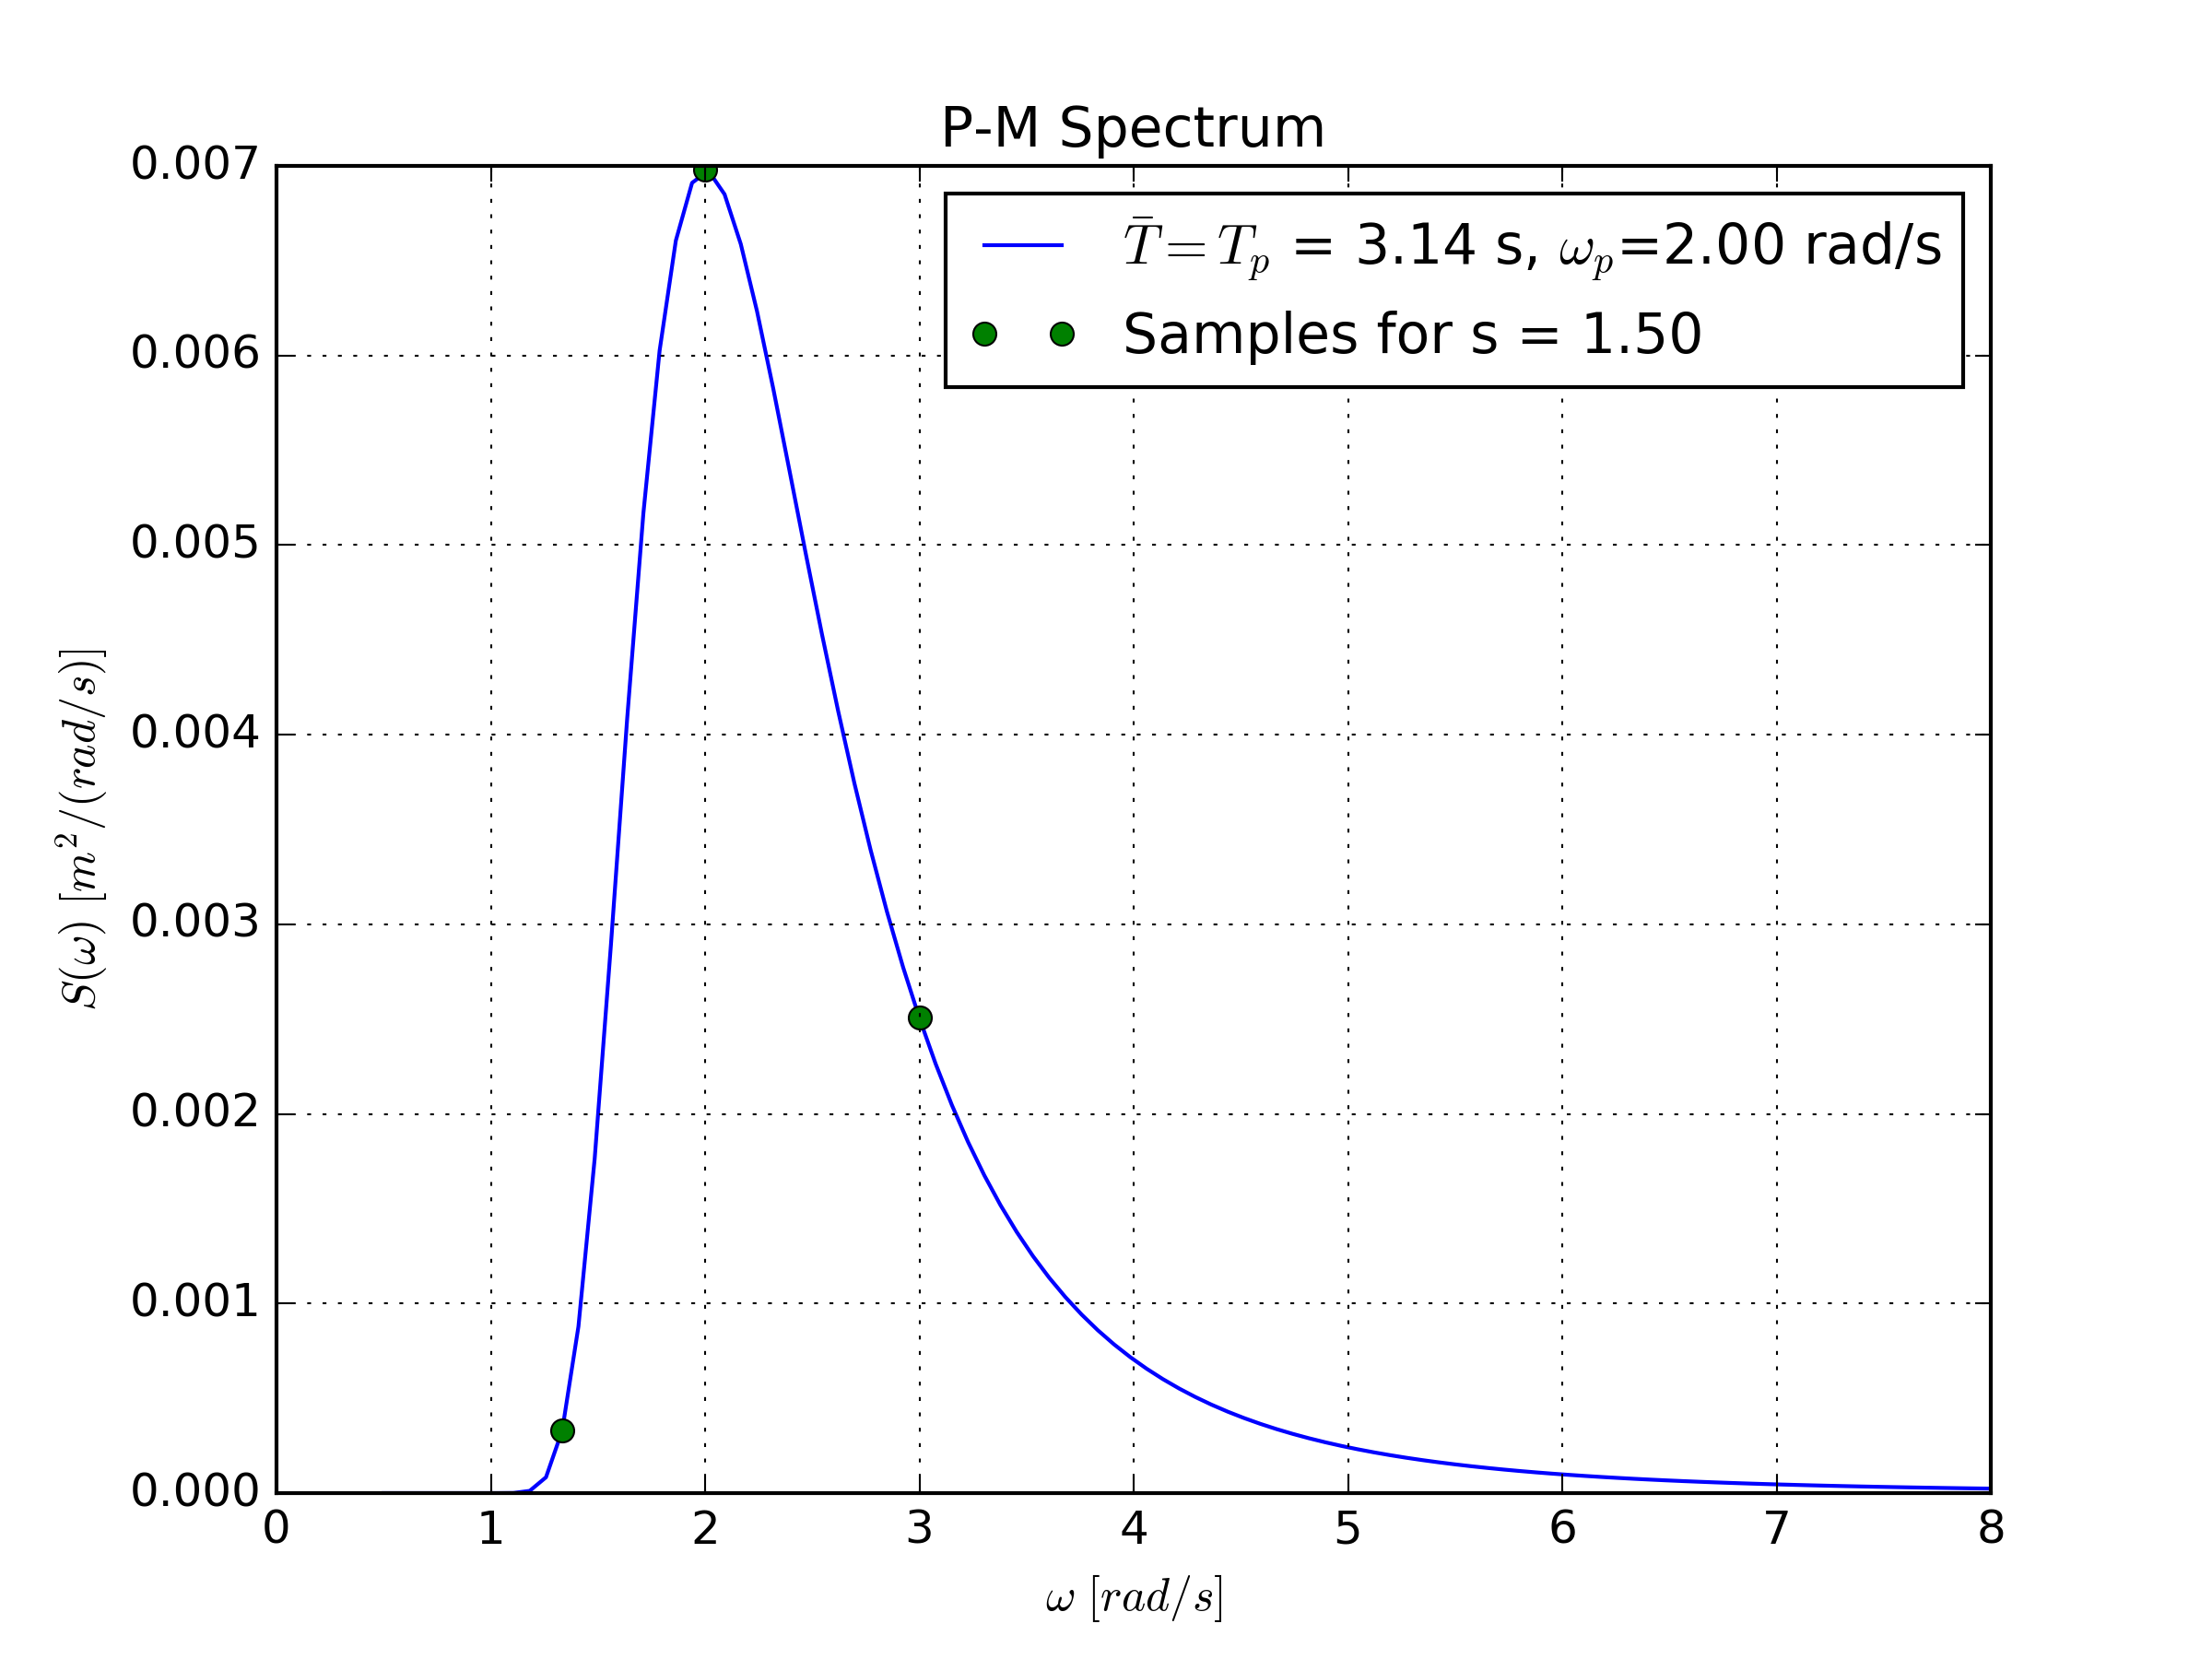
\includegraphics[width=0.8\textwidth]{pm_ex.png}}}
\caption{P-M spectrum example.}
\label{f:pm}
\end{figure}

The amplitude is determined from the spectrum by
\[
a_i^2 = 2 S(\omega_i) \Delta_i
\]
where $\Delta_i$ is the frequency spacing between samples. For $N=3$ this spacing is
\begin{eqnarray}
  i=0 & : & \Delta_0 = \omega_p(1-1/s) \\
  i=1 & : & \Delta_1 = \omega_p \frac{ s - 1/s}{s} \\
  i=2 & : & \Delta_2 = \omega_p (s-1).
\end{eqnarray}
We also include a gain value ($\gamma$) as a multiplier of the amplitude so that
\[
A_i = \gamma a_i = \gamma \sqrt{ 2 S(\omega_i) \Delta_i}
\]


\subsection{Constant Wavelength-Amplitude Ratio (CWR) Wavefield Model}

This model for generating the component waves is described in \cite{gpugems_waves}.  The general idea is that the user specifies the median wavelength and median amplitude.  The ratio of wavelength/amplitude is held constant, so longer wavelength/period waves tend to dominate the wave field. The median wavelength is specified indirectly via the median period, which is then used to calculate the median angular frequency and then the median wavenumber via the dispersion relationship.

\begin{algorithm}
  \caption{Constant Wavelength-Amplitude Ratio (CWR) Wavefield Model}
  \begin{algorithmic}
    \STATE $\bar{\omega} = \frac{2 \pi}{\bar{T}}$ (Median angular freq.)
    \STATE $\bar{k}= \frac{\bar{\omega}^2}{g}$ (Median wavenumber/lenght, via deep water dispersion)
    \STATE $i = 0$
    \FOR{$i<N$}
    \STATE $n=i - N/2$
    \STATE $A_i = \bar{A} (s^n)$
    \STATE $k_i = \frac{\bar{k}}{s^n}$
    \STATE $\omega_i = \sqrt{g k_i} = \bar{\omega}/ \sqrt{s^n}$
    \STATE $T_i = \bar{T} \sqrt{s^n}$
    \STATE $\Vi{d}{i} = \angle{(\theta_d + (n)(a))}$
    \STATE $\Vi{k}{i} = k_i \Vi{d}{i}$
    \STATE $q_i = \min{\{1.0, q/(A_i k_i N)\}}$
    \STATE $\phi_i = 0$
    \STATE $i++$
    \ENDFOR
  \end{algorithmic}
\end{algorithm}

\newpage
%\setcounter{page}{1}
\bibliographystyle{ieeetr}
\bibliography{refs}

\end{document}
